\label{chpt:modelling and techniques} % for referencing this chapter elsewhere, use 
\lhead{\emph{Modelling, techniques, and methods}} % This is for the header on each page - perhaps a shortened title

The primary goal of this thesis is to characterise as many CVs as possible, meaning to find the donor mass and radius, measurements of the white dwarf mass and radius, and the orbital separation between the two bodies. These metrics provide valuable probes of CV evolution \citep{knigge2006}, which is explored more thoroughly in \S\ref{sect:method:evolutionary modelling}. 
This chapter describes in detail the two modelling techniques used for this thesis: the characterisation of a CV using multi-band eclipse modelling, and inferring the long-term mass loss rate of a system from its donor properties. 
When fitting models to observations, the choice of algorithm is important. The majority of the parameter optimisation done in this work uses a type of Markhov Chain Monte Carlo (MCMC) technique, and this is also described in detail.


\section{Parameter optimisation}
Frequently in this work, a model must have its input parameters fit to observed or synthesised data. For models with few input parameters and well-behaved evaluation metrics, simple optimisation is possible, but often models have many parameters; for example the eclipse modelling portion of this work (\S\ref{sect:modelling:eclipse modelling}) has 18 parameters for a single eclipse, and fitting a full dataset frequently involves fitting 100 or more parameters. To make matters worse, the eclipse model is fairly expensive to compute in large numbers, making simple methods, like downhill simplex, untenable. Rather, we use MCMC.

The MCMC method is now a well-established tool in astronomy. It is robust, efficient, and yields the probability distribution of the variables being optimised even when not well-described by simple distributions. This has led to MCMC often being the method of choice when fitting models. 
This section provides a working knowledge of MCMC, but for an in-depth introduction and review of the technique and its various sub-types see \citet{sharma2017}. 

\subsection{Bayesian analysis}
Bayesian inference uses known, `prior' knowledge combined with new information to derive a better understanding - the `posterior' knowledge of a model. This somewhat self-evident intuition was formalised by Bayes with Bayes' Theorem, which calculates the probability, $p(H | D, I)$ a model, $H$, given some observed data, $D$, and background information, $I$. 
\begin{equation}
    \label{eqn:modelling:bayes symbolic}
    p(H | D,I) = \frac{p(D | H, I) \cdot p(H | I)}{p(D|I)}
\end{equation}
Here, $p(D | M, I)$ is the probability of the observed data, given a model and prior information, so is called the Likelihood, $\mathcal{L}$, of the data. 
$p(M|I)$ is the probability of the model being valid, given some prior information, so is called the prior distribution. $p(D | I)$, or the probability of observing the data, given the previously known information, is also called the the `Evidence', and acts as a normalisation factor. Using this vocabulary, Equation~\ref{eqn:modelling:bayes symbolic} can be written as:
\begin{equation}
    \label{eqn:modelling:bayes english}
    \rm Posterior = \frac{Likelihood \times Prior}{Evidence}
\end{equation}

\subsection{MCMC optimisation}
The MCMC is a tool developed to approximate the distributions in Equation~\ref{eqn:modelling:bayes symbolic}, without the need to process them analytically -- a process that quickly becomes prohibitively difficult as the number of variables increases. 
An MCMC, as the name suggests, is a combination of a Monte Carlo method, a class of algorithms that rely on random sampling to find a result, and a Markov chain, a mathematical system that transitions between states according to probabilistic rules. An MCMC randomly draws samples from the prior distributions of the model variables (the Monte Carlo half of the algorithm), evaluates their $\mathcal{L}$, and either accepts them onto its chain of sampled points or not, depending on if they meet a set of conditions. As the number of samples increases, the distribution of samples on the MCMC chain approaches the `true' distribution of the model variables, given a set of observations. 

When optimising parameters for a model, different sampling methods are used for different situations. 
The most basic of these sampling methods is the Metropolis-Hastings (M-H) algorithm \citep{metropolis1953,hastings1970}. 

For each step in the chain, a parameter vector, $\theta_i$, is chosen at random from a proposal distribution $q(\theta_i | \theta_{i-1})$. The likelihood of observing data $D$, $\mathcal{L}_i(D | \theta_i)$ is evaluated; conveniently, $\mathcal{L}$ is related to the $\chi^2$ metric by $\mathcal{L} \propto \mathrm{exp}(-\chi^2/2)$, so the change in $\mathcal{L}$ is relatively easy to compute.

Then, $\theta_i$ is either accepted or rejected from the chain depending on the current state of the chain. If the $\mathcal{L}_i > \mathcal{L}_{i-1}$, i.e. the $\mathcal{L}$ has improved, the sample is accepted. However, if $\mathcal{L}_i < \mathcal{L}_{i-1}$, the acceptance is determined by the transition probability, $P(\theta_i | \theta_{i-1})$, defined as 
\begin{equation}
    P(\theta_i | \theta_{i-1}) = \alpha(\theta_i | \theta_{i-1}) \cdot q(\theta_i | \theta_{i-1})
\end{equation}
where $\alpha(\theta_i | \theta_{i-1})$ is the acceptance probability, 
\begin{equation}
    \alpha(\theta_i | \theta_{i-1}) = \frac{P(\theta_i | D)} {P(\theta_{i-1} | D)} \cdot \frac{q(\theta_{i-1} | \theta_i)} {q (\theta_i | \theta_{i-1})}
\end{equation}
In other words, the larger the drop in probability, the \textit{less likely} it is to accept $\theta_i$ onto the chain. This finite chance to accept a new point, even if it is less likely to describe the data, makes the chain \textit{reversible}, and allows the algorithm to explore the full alloable parameter space (given an infinite number of steps) even if doing so first requires moving to a less preferred $\theta$. 


\section{Finding an orbital ephemeris}
\label{sect:modelling:getting ephemeris}

Crucial to both observing and modelling an eclipse is a good knowledge of the orbital ephemeris. This is described by the equation
\begin{equation}
    \label{eqn:modelling:general ephemeris equation}
    T_{\rm ecl} = T_0 + P_{\rm orb} E
\end{equation}
where $T_{\rm ecl}$ is the time of mid-eclipse, $T_0$ is the mid-eclipse time of the zeroth eclipse, and $E$ is the eclipse number. Accurately calculating $T_{\rm ecl}$ is important to scheduling observations of a system, and $P_{\rm orb}$ is a crucial to the eclipse modelling. 

As observations are often separated by several months or even years, an error in $P_{\rm orb}$ of even $\sim 0.1$ seconds can accumulate to give significantly inaccurate predicted eclipse times. This need for precision also requires the definition of {\it where} a time is recorded from. All eclipse times presented in this thesis are given in the Barycentric Modified Julian Date (BMJD), which is the time of eclipse as measured from the centre of mass of the solar system. Note that this is different to the heliocentric MJD often seen in the literature, and where heliocentric literature values are used, they are first converted to BMJD. 

\subsection{Finding eclipse times}
\label{sect:modelling:finding eclipse times}

When finding an eclipse time, simply taking a time of minimum light is insufficient for the systems in this work. This is because it is common for CV eclipses to have very flat eclipse minima, and because CV eclipses have a fairly complex structure. 
A somewhat more sophisticated method is necessary, and finding the mid-eclipse time is done by looking at the numerical derivative of an eclipse. 
First, an eclipse is smoothed to remove short term fluctuations, partly those due to noise but also to mitigate the short term flickering often seen in CVs. This initial smoothing is done by applying a median filter to the data. Then, the numerical derivative is calculated and smoothed again, this time with a `boxcar' convolution. Properly filtered, the dominant remaining features of the numerical derivative are the ingresses and egresses of the white dwarf and bright spot. 
The white dwarf ingress and egress are, in theory, symmetrical -- the ingress should be a sharp, negative spike, and egress should be a sharp, positive spike. As the two should be the same shape, a double-gaussian is fit to the derivative, using manually chosen initial conditions. In this model, the two gaussians share a width, $\sigma$, and have their mid-points described by
\begin{align*}
    T_{\rm 1,2} = T_{\rm ecl} \pm \Delta T \\
    h_{\rm 1,2} = \pm h
\end{align*}
where $T_{1,2}$ are the respective midpoints of the two gaussians, $h_{1,2}$ are their respective heights, and $2\Delta T$ is the distance between the two gaussians. 
The derivative is then fit with these free parameters using an MCMC, to give the $T_{\rm ecl}$.

\subsection{Computing period}
\label{sect:modelling:Computing ephemeris}

To find a rough initial ephemeris of a system, at least two eclipse observations with known $E$ are necessary. Given no prior knowledge of $P_{\rm orb}$ and $T_0$, this can be done by simply observing the system for several hours, until two consecutive eclipses are seen. This gives a rough measure of $P_{\rm orb}$, but can be significantly refined with longer baseline observations. 
For each observed $T_\mathrm{ecl}$, $E$ could unambiguously be determined, either from observing consecutive eclipses or from previously reported literature values.
An MCMC algorithm was used to fit a straight line model to the independent variable $E$\ and dependent variable $T_\mathrm{ecl}$, with a gradient $P$\ and intercept $T_0$. 
The model also accounts for potential systematic differences in timing accuracy between instruments by also having variable error scale factors applied to all eclipses observed with a specific instrument, e.g. the timing reported for eclipses observed with ULTRACAM may be systematically offset from reality, and the errors associated with those observations might need to be larger than reported to be consistent with data from other instruments. The prior distribution assumed for these error factors was log-uniform ranging from 0.01 to 100, which favours the smallest factor consistent with the data. 

The value of $E$ for each eclipse were chosen to minimise the covariance between $T_0$ and $P$. 
% If we consider the result of fitting  $T_0, P_{\rm orb}$ as a multivariate normal, $N(\mu, \Sigma)$, we can write
% \begin{align}
%     \mu =& 
%     \begin{pmatrix}
%         T_0 \\
%         P_{\rm orb}
%     \end{pmatrix}
%     \\
%     \label{eqn:modelling:ephemeris multivariate normal}
%     \Sigma =& 
%     \begin{pmatrix}
%         \sigma_{\rm T0}^2 & \sigma_{\rm T0} \sigma_{\rm P} \\
%         \sigma_{\rm P} \sigma_{\rm T0} & \sigma_{\rm P}^2  \\
%     \end{pmatrix}
% \end{align}
Consider a predicted eclipse time for $E$. The uncertainty on $T_{\rm ecl}$ in Equation~\ref{eqn:modelling:general ephemeris equation} can be written as,
\begin{equation}
    \sigma_{T{\rm ecl}}^2 = \sigma_{\rm T0}^2 + 2\sigma_{\rm T0} \sigma_{\rm P}E + \sigma_{\rm P}^2 E^2
\end{equation}
from the standard error propagation formula.
To evaluate an alternative set of $E$, $E$ can be offset by some integer, $N$, with $E' = E - N$. Then, by expanding out the brackets and consolidating some terms, $\sigma_{T{\rm ecl}}^2$ becomes
\begin{align*}
    \sigma_{T{\rm ecl}}^2 =& \sigma_{\rm T0}^2 + 2\sigma_{\rm T0} \sigma_{\rm P}(E'+N) + \sigma_{\rm P}^2 (E'+N)^2 \\
    =& (\sigma_{\rm T0}^2 + \sigma_{\rm P}^2 N^2 + 2\sigma_{\rm T0} \sigma_{\rm P} N) + 2(\sigma_{\rm T0} \sigma_{\rm P} + \sigma_{\rm P}^2 N)E' + \sigma_{\rm P}^2 E'^2
\end{align*}
Since we want to minimise the $\sigma_{T{\rm ecl}}^2$ term, we can choose a value of $N$ to do so, $N = -(\sigma_{\rm T0}\sigma_{\rm P})/(\sigma_{\rm P}^2)$ rounded to the nearest integer.


\section{Characterising a CV}
\label{sect:method:lightcurve modelling}

To determine the system parameters for the three CVs in this study, the eclipse lightcurves were modelled. This method is more frequently applicable in CVs than the more traditional approach of using spectroscopic eclipsing binaries, since the donor star is rarely directly visible. Compared to using the superhump period excess to estimate the mass ratio \citep{patterson2005, knigge2006}, lightcurve modelling requires few assumptions. However, it does require precise alignment of the system and so is not possible for a large fraction of CVs.

CV eclipse modelling was first developed by \citet{wood1986}, and has been refined significantly over the last decade \citep{Savoury2011, McAllister2017, McAllister2019}. This method relies of four assumptions: \textit{(1)} the stream of mass flowing from the donor to the white dwarf follows a ballistic trajectory, \textit{(2)} the white dwarf obeys a theoretical mass-radius relationship, \textit{(3)} the white dwarf is unobscured by the accretion disc or other sources of intra-system material, and \textit{(4)} the donor exactly fills its Roche lobe. Most of these assumptions are considered robust, though the visibility of the white dwarf been called into question by \citet{Spark2015}.

Assuming that the secondary star completely fills its Roche lobe (which is required for mass transfer) ensures that the donor radius is solely a function of $q$. The white dwarf eclipse width is set by the width of the donor, the separation between the two stars, and $q$. The width of the white dwarf eclipse, therefore, is solely a function of $q$, $P_{\rm orb}$, and inclination, $i$ \citep{bailey1979}. 

Assuming that the mass stream between the two stars follows a ballistic trajectory that follows a path determined by $q$ \citep{Lubow1975}, the location of the bright spot can be fixed in space as the point at which the ballistic stream intersect the outer edge of the accretion disc. Therefore, the phase of the bright spot ingress and egress is a function of $q$, and the disc radius. 

Assuming that the white dwarf is unobscured allows us to directly relate the inclination, and the duration of ingress and egress to the white dwarf's radius. Because the white dwarf is assumed to follow a known mass-radius relationship, by fitting the observed white dwarf colours with a temperature, gravity, distance and interstellar extinction, the temperature and radius of the white dwarf yield a mass. The donor mass is then a simple product of the white dwarf mass, and $q$.

The final result of modelling is the following parameters,
\begin{itemize}
    \item white dwarf and donor masses
    \item white dwarf and donor radii
    \item orbital separation
    \item orbital velocity of the white dwarf and donor
    \item inclination
    \item white dwarf effective temperature and surface gravity
    \item distance
\end{itemize}

The modelling actually takes place in two phases, which are each described in detail - first the phase-folded eclipse is modelled, then the resulting proxy variables are converted to physical parameters. \todo{Put in some history here -- old versions using the derivative, comparison with other methods, past analysis with this method.}

\subsection{Phase-folded eclipse modelling}
\label{sect:modelling:eclipse modelling}

Recall that the light from a CV originates from four distinct objects in the system. The white dwarf and donor star, the accretion disc about the white dwarf, and the bright spot impact region (hereafter simply `the bright spot'), where transferred material impacts the outer rim of the accretion disc and liberates significant amounts of energy. Notably the bright spot emits flux directionally, so 
The anatomy of a CV eclipse lightcurve is a sequence of five events, that occur in the following order:
\begin{enumerate}
    \item a pre-eclipse hump is often seen as the bright spot rotates into view
    \item The white dwarf becomes obscured by the donor
    \item The bright spot becomes obscured by the donor
    \item The white dwarf emerges from behind the donor
    \item The bright spot emerges from behind the donor
\end{enumerate}
Figure\todo{Make a figure for this} shows a typical lightcurve, with these events marked. 

The model schematic of a CV in \lstinline{lfit} is shown in Figure\todo{make a schematic for this -- labelled!}. At this stage, parameters are not yet in SI units, which is done to make the modelling software more efficient. Rather, the phase-folded lightcurve is generated, causing parameters to be scaled, i.e. $q$ is fit rather than masses directly, and distances are scaled to the distance from the white dwarf primary to the $L_1$ point, $x_{l1}$
A single eclipse is described by 18 parameters:
\begin{itemize}
    \item White dwarf, donor star, disc, and bright spot fluxes, $F_{\rm wd,\ donor,\ disc, bs}$
    \item Mass ratio, $q$
    \item White dwarf eclipse width in units of phase, $\Delta \phi$
    \item Scaled white dwarf radius, $R_{\rm wd} / x_{l1}$
    \item White dwarf limb darkening coefficient, $u_{\rm ld}$
    \item Scaled outer disc radius, $R_{\rm disc} / x_{l1}$
    \item Disc surface profile exponent, $b$
    \item Seven parameters describing the bright spot
    \item An eclipse phase offset, $\phi_0$
\end{itemize}
The seven bright spot parameters are not physically motivated, but relate to the bright spot model. 

\subsubsection{The white dwarf model}

The white dwarf is modelled as a disc, with a total surface brightness $F_{\rm wd}$ and a radius of $R_{\rm wd} / x_{l1}$. It is subject to limb darkening, using a linear prescription:
\begin{equation}
    \frac{I_l}{I_0} = 1 - u_{\rm ld}(1 - {\rm cos}\beta)
\end{equation}
where $I_0$ is the intensity at the centre of the disc, and $I_l$ is the intensity at a limb. $\beta$ is the angle between the line normal to the surface of the white dwarf, and the observer's line of sight. 

\subsubsection{The donor star}
The secondary star does not become obscured during an eclipse, but there is some variation in its brightness. The donor is not spherical, so a small ellipsoidal variation is seen as it rotates to expose more or less of its surface to the observer.

\subsubsection{The accretion disc}
The accretion disc is modelled as a series of annular rings about the white dwarf, extending out to $R_{\rm disc} / x_{l1}$. The intensity of each annulus decreases with distance from the white dwarf, following an exponential formula, $I_i \propto R^{-b}$ for ring $i$ at distance $R$ from the white dwarf. As $b$ is a free parameter in the model, discs can be made more or less centrally concentrated to match observations. As the bright spot location is determined by $q$ and $R_{\rm disc} / x_{l1}$, the phases of bright spot ingress and egress provide a valuable diagnostic for $R_{\rm disc} / x_{l1}$.

\subsubsection{The bright spot}
The bright spot model is not physically motivated, but rather is chosen to be able to reproduce a large range of bright spot eclipses. 
It is modelled as a strip of flux extending in both directions tangentially from the edge of the disc, with a defined brightness profile and overall flux. The strip intensity falls off exponentially, described by the equation
\begin{equation}
    I_{\rm X} \propto \bigg ( \frac{X}{S} \bigg )^Y \cdot {\rm exp} \bigg [ - \bigg (\frac{X}{S} \bigg )^Z \bigg]    
\end{equation}
where $I_{\rm X}$ is the intensity of the strip a distance $X$ along it, and $S$ is the scale of the bright spot. $Y$ and $Z$ are the profile exponents. 

The bright spot is known to emit light directionally, at a beaming angle, $\theta_{\rm yaw}$, from the normal to the strip in the plane of the disc, and an angle $\theta_{\rm tilt}$ from the plane of the disc. 
Some fraction of the light is beamed, and the rest, $f_{\rm is}$, is emitted isotropically from the strip. This geometry is shown in Figure~\ref{fig:modelling:bright spot schematic}
\begin{figure}
    \centering
    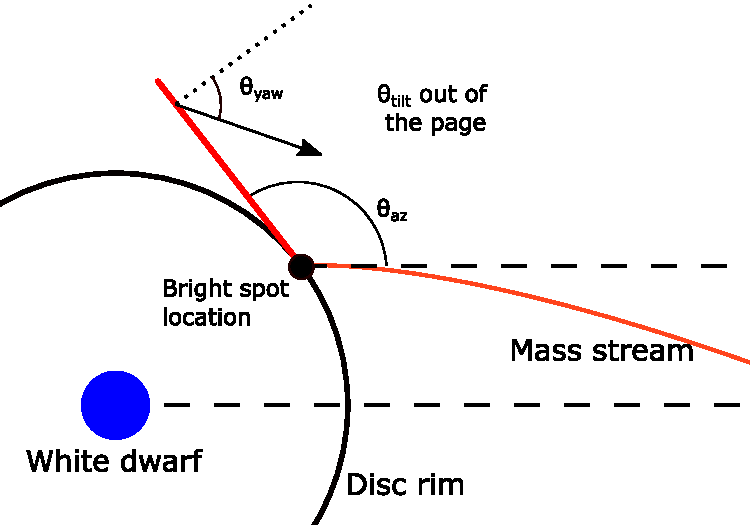
\includegraphics[width=0.9\textwidth]{figures/modelling/bright_spot_schematic.pdf}
    \caption{Showing a schematic of the bright spot model. The lower dashed line joins the centres of the white dwarf and donor stars, and the upper dashed line runs parallel to it, intersecting the bright spot location. The thick red line is the flux-emitting strip, and the arrow shows the direction of light emission, at an angle $\theta_{\rm yaw}$ from the normal.}
    \label{fig:modelling:bright spot schematic}
\end{figure}

Lower values of $q$ will cause the ballistic stream to take a wider arc towards the white dwarf, moving the intersection point with the disc. The location of the bright spot on the disc edge is defined by $\theta_{\rm az}$, the angle between the strip and the line of sight of the observer.

As the bright spot is the most complex component of the model, there is an option to simplify it in software for systems with faint bright spot features that cannot be properly resolved.
This mode is called the `simple' bright spot model, and fixes $\theta_{\rm tilt}$ at $90\deg$, $\theta_{\rm yaw}$ at $0\deg$, and the strip exponents $X$ and $Y$ to 1 and 2, respectively. By removing these four degrees of freedom, better characterisation of the eclipse is possible.

\subsection{Post-processing the eclipse model}
\label{sect:modelling:post processing the eclipse model}

The eclipse modelling uses proxy variables, so some processing must be done to convert them to `real' values. This is done in two steps. First, the white dwarf colours are fit to find a white dwarf temperature and surface gravity. Then, the white dwarf temperature and orbital period are combined with the best-fit eclipse model parameters to convert the scaled distances to metres, and mass ratio to kilograms. 

\subsubsection{Fitting white dwarf colours}
\label{sect:modelling:fitting white dwarf colours}
By modelling the eclipse in multiple bands, at least three observations of white dwarf flux are available. These fluxes are fit to the DA white dwarf cooling model from \citet{Bergeron1995}\footnote{Available from \href{http://www.astro.umontreal.ca/~bergeron/CoolingModels}{http://www.astro.umontreal.ca/~bergeron/CoolingModels}}, from which the absolute magnitude of the white dwarf in each band, $M$, can be retrieved from pre-calculated cooling tracks for a given effective temperature, $T_{\rm eff}$ and surface gravity, $\mathrm{log(g)}$. This absolute magnitude is then easily translated to an apparent magnitude, $m$, given a system parallax, $\pi$, and interstellar extinction coefficient, $\rm E(B-V)$,
\begin{equation}
    m = M - 5\mathrm{log}(\pi\mathrm{,\ arcsec}) - 5
\end{equation}

To optimise these four parameters, an affine-invariant MCMC with three levels of parallel tempering was used, c.f. \S\ref{sect:modelling:ensemble MCMC}. For the priors, uniform $T_{\rm eff}$ and log($g$) distributions were used that span the range set by the model cooling tracks. $\rm E(B-V)$ used a uniform distribution between 0, and the maximum IRSA measurement for the relevant coordinates\footnote{Available \href{https://irsa.ipac.caltech.edu/applications/DUST/}{https://irsa.ipac.caltech.edu/applications/DUST/}}, and the parallax prior was chosen to match the Gaia measurement \citep{lindegren2018, Luri2018, Gaia2016, Gaia2018} of the system. 

\subsubsection{Conversion of proxy variables to physical parameters}
\label{sect:modelling:conversion to physical parameters}
The eclipse model proxy variables are then converted to real values. This is done using the white dwarf as a known quantity, based on white dwarf model atmospheres. Five input variables are needed: $T_{\rm eff}$, $P_{\rm orb}$, $q$, $\Delta \phi$, and $R_{\rm wd} / x_{l1}$.


A measure of the white dwarf radius, $R_{\rm wd}$, can be found using Kepler's 3rd law and making the substitutions $r = R_{\rm wd} / a$ and $q = M_{\rm wd} / M_{\rm donor}$. 
\begin{align}
    P_{\rm orb}^2 &= \frac{4 \pi^2 a^3}{G (M_{\rm wd} + M_{\rm donor})} \\[8pt]
    &= \frac{4 \pi^2 R_{\rm wd}^3}{G M_{\rm wd} (1 + q) r^3} \\[8pt]
    R_{\rm wd}^3 &= \frac{P_{\rm orb}^2 r^3 G M_{\rm wd} (1 + q) }{4 \pi^2}
    \label{eqn:modelling:geometric radius}
\end{align}
$r$ can be found from $R_{\rm wd} / x_{l1}$ by calculating $x_{l1} / a$, which itself is a function only of $q$. 

This value of $R_{\rm wd}$ is geometric mass-radius relationship, and requires the white dwarf mass. Fortunately, for a given $T_{\rm eff}$ (which is known from the colour fits, \S\ref{sect:modelling:fitting white dwarf colours}), white dwarfs follow tight theoretical mass-radius relationships, that can be employed to find the unique $M_{\rm wd},\ R_{\rm wd}$ pair that satisfies both Equation~\ref{eqn:modelling:geometric radius} and the theoretical mass-radius relationship. 
Specifically, a proposed theoretical mass-radius pair is chosen from a model relationship and a value of $R_{\rm wd, calc}$ is calculated from Equation~\ref{eqn:modelling:geometric radius}. If this matches the theoretical value, the mass is valid. Otherwise, the proposed mass is altered accordingly and a new mass-radius pair is checked. 

Three white dwarf mass-radius relations were used. First, a solution was searched for using the \citet{wood1995} models, spanning masses of $0.4 - 1.0 M_\odot$. 
If no solution could be found, the \citet{panei2000} models were searched, spanning masses from $0.4 - 1.2 M_\odot$. 
Both of these mass-radius relationships account for the white dwarf $T_{\rm eff}$. However, if no solution has been found, the \citet{hamada1961} 0 Kelvin mass-radius relation is checked for solutions. This track spans the largest range in mass, from $0.14 - 1.44 M_\odot$. If no solution is found with the \citet{hamada1961} tracks, the model is considered invalid, though this did not occur for any system in this thesis.

Then, the inclination is calculated. $\Delta \phi$ is solely a function of $q$, and $i$. Therefore, we can use the known values of $\Delta\phi$ and $q$ to calculate the system inclination - this is done by proposing candidate values of $i$, and comparing the calculated $\Delta \phi_{\rm calc}$ with the target $\Delta \phi$, and adjusting as needed until the two agree.  

Now, three quantities are known; $i$, $M_{\rm wd}$, and $R_{\rm wd}$. As previously mentioned, $R_{\rm donor}$ is assumed to be the Roche radius, from Equation~\ref{eqn:introduction:eggleton approximation}, and $M_{\rm donor}$ is found simply by $(q \cdot M_{\rm wd})$. Finally, the orbital velocities, $K_{\rm wd,\ donor}$ respectively, of the two stars are calculated using Kepler's laws.
\begin{align}
    K_{\rm wd} &= \frac{2\pi a \mathrm{sin}i}{P_{\rm orb}} \frac{q}{1+q} \\
    K_{\rm donor} &= K_{\rm wd} \cdot \frac{M_{\rm wd}}{R_{\rm wd}}
\end{align}


\subsection{Capturing flickering with Gaussian Processes}
Explain GPs from scratch, and get into detail about which kernels you're using. 


\subsection{Hierarchical model structure}
{\bf This is going to take some work. Fit synthetic lightcurves with various amounts of noise, (5\%, 10\%, 20\%?), and compare convergence times and posterior widths as a function of noise. Do this with one eclipse, then with three eclipses of the same band, then with three eclipses in each of three bands.
I should see an improvement in final probability distribution with more eclipses, since they can communicate.
Also, I need to come up with a way to demonstrate the potential to break degeneracies. Some lightcurves might be produced by two different parameter vectors, e.g. disc and donor might look similar to each other. }

I extend the lightcurve fitting model used by \citet{McAllister2019}, adopting a hierarchical approach to slightly reduce model complexity. 

Changes in the disc radius and brightness profile, and bright spot parameters can mean that the same CV has a significantly different eclipse lightcurve at different times, making it difficult to justify averaging together many eclipses, as features can become smeared out and uninformative. In the worst-case scenario, all 18 parameters would be independently variable for each eclipse, in each band. However, by sharing some parameters between eclipses and bands, this large number of free parameters is slightly reduced, and the posterior of some parameters can be informed by multiple eclipses. \citet{McAllister2017} share $q,\ R_{\rm wd} / x_{l1}$, and $\Delta\phi$ between eclipses, and we extend that concept by organising the model into a hierarchical tree structure, a schematic of which is shown in Figure~\ref{fig:method:hierarchical_model}. 

\begin{figure}
    \centering
    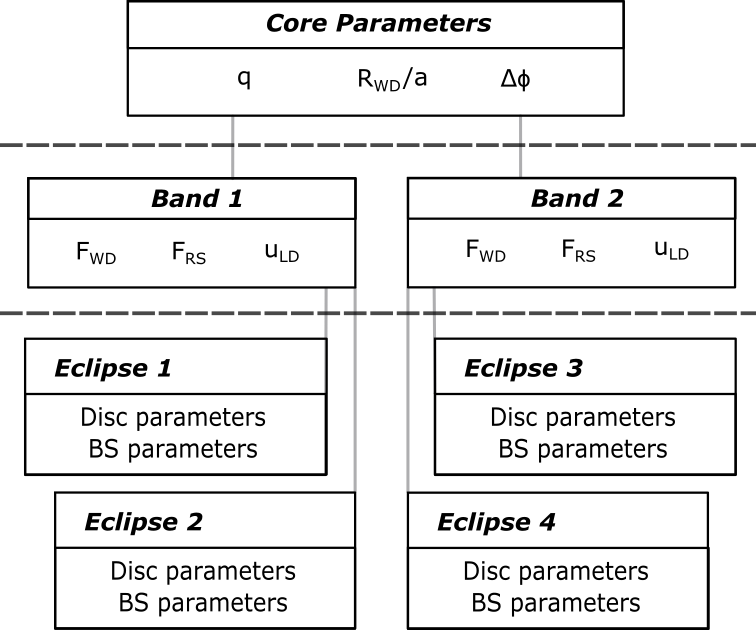
\includegraphics[width=.85\columnwidth ]{figures/three_cvs_with_weird_colours/GeneralFigs/hierarchical_model_structure.png}
    \caption{The hierarchical structure of the lightcurve model. Parameters are inherited downwards, to produce an eclipse at the `leaves' of the tree, e.g. Eclipse 3 inherits the parameters of Band 2, which in turn inherits the Core parameters. $\mathrm{F_{WD, RS}}$\ represent the fluxes of the white dwarf and donor star, and $\mathrm{U_{LD}}$\ is the limb darkening coefficient of the white dwarf.}
    \label{fig:method:hierarchical_model}
\end{figure}

The top level of the model provides the core parameters, which are unchanging between all observing bands and constant across our observations: $q,\ R_\mathrm{WD}/a$, and $\Delta\phi$. We assume the white dwarf and donor fluxes do not change on the timescale of our observations, and so these variables, along with the limb darkening coefficient of the white dwarf, are shared between all eclipses observed with the same filters. The bottom level holds parameters that can vary quickly enough to change between eclipses, i.e. parameters describing the accretion disc and bright spot. By handling parameters this way, we maximise the amount of data informing important variables, for example, white dwarf fluxes and $q$. We also somewhat reduce the number of free parameters, which aids slightly in model fitting, but the chief justification for the hierarchical approach is that it ensures consistency between eclipses - something not guaranteed when fitting eclipses individually.

As more eclipses are added, the number of dimensions in parameter space that must be explored increases. For illustration, the model for ASASSN-17jf has 3 eclipses across 3 bands, plus 3 Gaussian process parameters, resulting in 87 free parameters that must be optimised simultaneously. To find the most likely set of lightcurve parameters in this very large space, an ensemble MCMC fitting code was used. The MCMC uses the \texttt{emcee} implementation of an ensemble sampler and parallel tempering \citep{foreman2012} to aid convergence to a global minimum despite the large parameter space, as described in \citet{McAllister2019}.




\subsection{MCMC Fitting}
\label{sect:modelling:ensemble MCMC}

I need to talk about the MCMC aspect of the fitting. Obviously explain MCMC fitting from scratch, but also make sure you explain the stretch move thing, ensemble sampling, 

\subsubsection{Parallel Tempering}
Make sure you point out the downfall of PT - it's not suitable for more than 5 parameters! We seem to get away with it by using a lot of walkers, perhaps?


\section{Evolutionary modelling}
\label{sect:method:evolutionary modelling}